\section{Prototype} \label{sec:s1_prototype}
Based on the initial requirements and the related work we first developed a mock-up of the application. This mock-up was intended as a low fidelity presentation of the core idea for our application. This mock-up was used internally in the group, as a way to share and agree on ideas for the application. Additionally we expected that the mock-up would be used to present our ideas to potential users. This mock-up was based on Google Maps' API.

Since the meetings with potential users could not be scheduled as early as hoped, we decided to continue the development and create a more high fidelity prototype, with the aim of presenting this to potential users and getting their feedback on the system, and not only the idea. The focus of the prototype is on the functionality and usability of the system, and so the prototype will use simulated crowd data. Due to requirements S1-FR3 and S1-FR4 in \cref{tab:s1_req} of running on multiple platforms, the prototype was developed as a web-application.

The prototype system was imagined as the main source of information on the state of the crowd. According to requirement S1-FR1 in \cref{tab:s1_req}, the system should display the information on a map.

% server-klient, cross platform

\subsection{Initial System Architecture}
Requirements demand that the system should run on many devices simultaneously, and therefore, for this initial prototype, we developed the prototype to exist as a client in a client-server architecture. The initial architecture is illustrated in \cref{fig:init_architecture}. The client can receive position data from a server, which in turn communicates with the aSTEP platform. The Cisco and GPS nodes in the architecture diagram symbolises location data being transmitted to the aSTEP platform for storage and processing.

\begin{figure}[htbp]
    \centering
    \begin{tikzpicture}[
    clientNode/.style={circle, draw=black, thick, text width=12mm, align=center},
    serverNode/.style={rectangle, draw=black, thick, minimum size=5mm},
    ]
     
    \node[serverNode] (coreAPI) {aSTEP core API};
    \node[serverNode] (server) [above right=of coreAPI] {Server};
    \node[clientNode] (cisco) [above left=of coreAPI] {Cisco};
    \node[clientNode] (client) [above=of server] {Client};
    \node[clientNode] (mobileGPS) [above=of coreAPI] {GPS};
    
    \draw[thick]
    (cisco.south) -- (coreAPI.north)
    (mobileGPS.south) -- (coreAPI.north)
    (client.south) -- (server.north)
    (server.south) -- (coreAPI.north);
    
    \end{tikzpicture}
    \caption{Initial architecture.}
    \label{fig:init_architecture}
\end{figure}


In order to fulfil the requirements S1-FR3 and S1-FR4 in \cref{tab:s1_req}, the prototype was chosen to be a web-application, since it would only require the target platform to support common web technologies such as HTML and JavaScript.

\subsection{Visualisation}
Different information can be important depending on the situation. In order to avoid information overload, the concept of toggleable overlays of information was employed, such that an operator can customise the information displayed. On \cref{fig:prototype1,fig:prototype2} the different information layers can be seen. \Cref{fig:prototype1} only shows the density layer, where \cref{fig:prototype2} also has an additional turbulence overlay activated.

\begin{figure}[htbp]
\centering
\begin{subfigure}{.48\textwidth}
    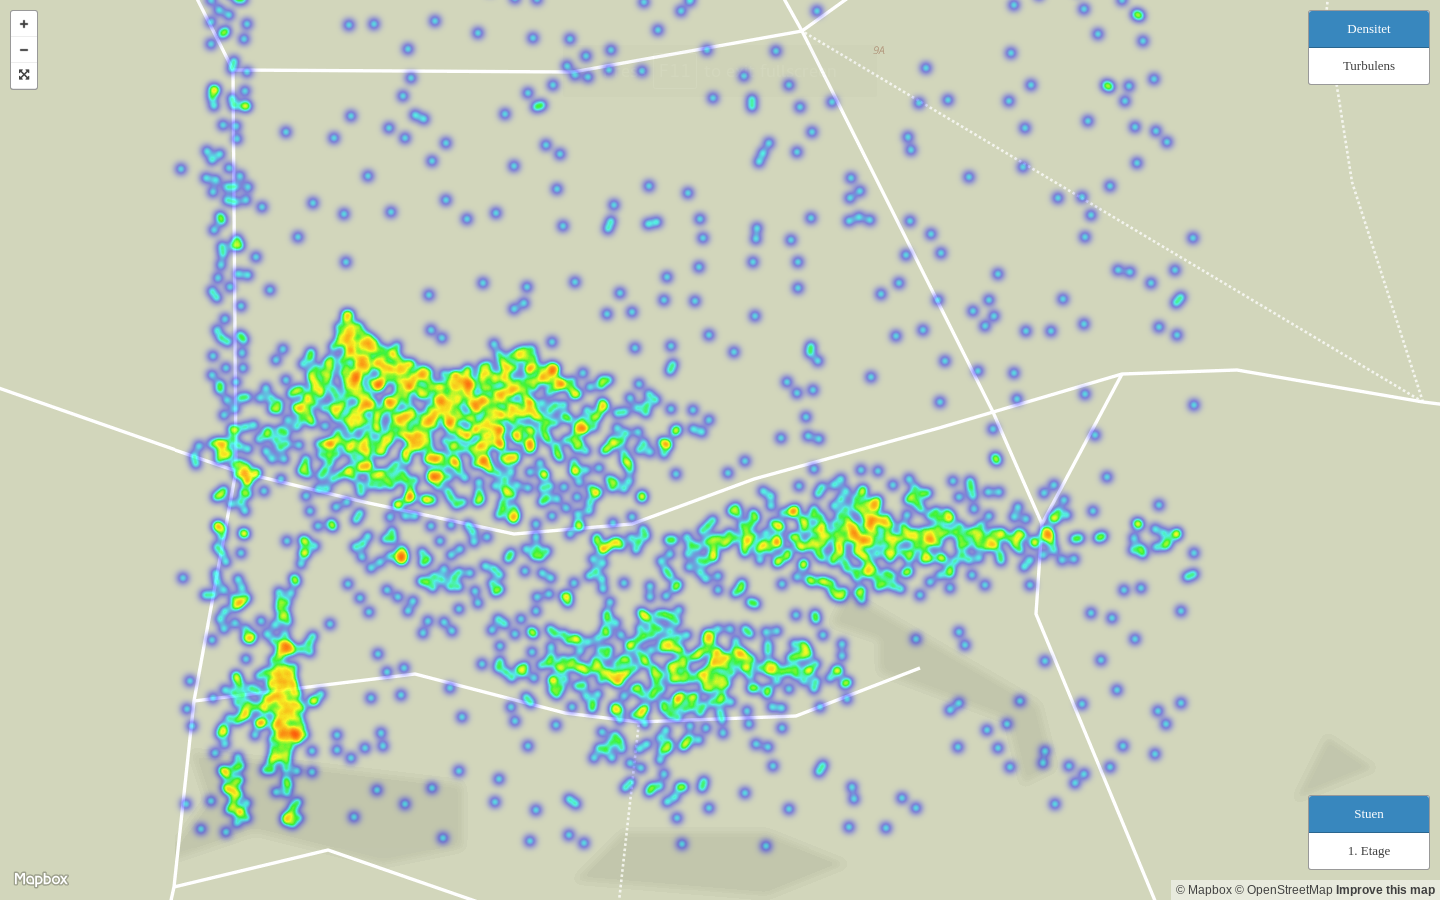
\includegraphics[width=\textwidth]{prototype1}
    \caption{With density overlay.}\label{fig:prototype1}
\end{subfigure}
\quad % spacing
\begin{subfigure}{.48\textwidth}
    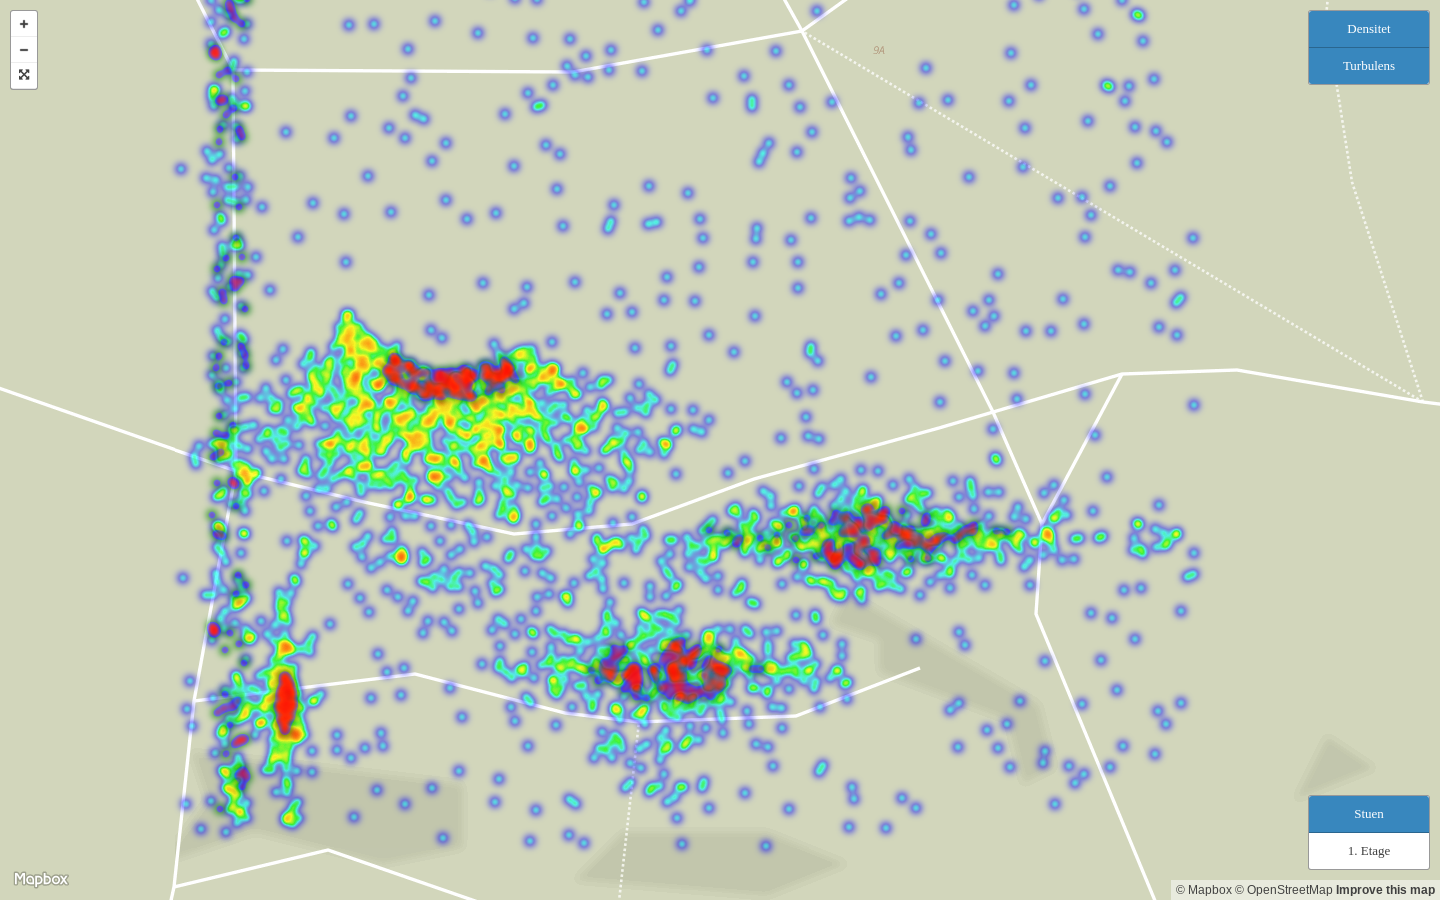
\includegraphics[width=\textwidth]{prototype2}
    \caption{With density and turbulence overlays.}\label{fig:prototype2}
\end{subfigure}
\caption{Screenshots of the first prototype.}
\end{figure}

The information displayed in the prototype is inspired by related work described in \cref{sec:related_work}. Specifically the prototype displayed here shows simulated density and turbulence at the main stage of the SmukFest festival. The colour scheme ranges from blue to red, representing low and high densities, respectively. The positions displayed in the prototype moved around in a pseudo-random pattern to give the impression of movement being shown in near real-time.